\documentclass[dvisvgm,hypertex,aspectratio=169]{beamer}
\usefonttheme{serif}

%\usepackage[draft]{animate}
\usepackage[final]{animate}
\usepackage{ifthen}


%%%%%%%%%%%%%%%%%%%%%%%%%%%%%%%%%%%%%%%%%%%%%%%%%%%%%%%%%%%%%%%%%%%%%%%%%%%%%%%
% PageDown, PageUp key event handling; navigation symbols
%%%%%%%%%%%%%%%%%%%%%%%%%%%%%%%%%%%%%%%%%%%%%%%%%%%%%%%%%%%%%%%%%%%%%%%%%%%%%%%
\usepackage[totpages]{zref}
\usepackage{atbegshi}
\usepackage{fontawesome}
\setbeamertemplate{navigation symbols}{}
\AtBeginShipout{%
  \AtBeginShipoutAddToBox{%
    \special{dvisvgm:raw
      <defs>
      <script type="text/javascript">
      <![CDATA[
        document.addEventListener('keydown', function(e){
          if(e.key=='PageDown'){
            \ifnum\thepage<\ztotpages
              document.location.replace('\jobname-\the\numexpr\thepage+1\relax.svg');%
            \fi
          }else if(e.key=='PageUp'){
            \ifnum\thepage>1
            %document.location.replace('\jobname-\the\numexpr\thepage-1\relax.svg');%
              document.location.replace('\jobname-\makeatletter\@anim@pad{2}{\thepage-1}\makeatother\relax.svg');%
            \fi%
          }
        });
      ]]>
      </script>
      </defs>
    }%
  }%
  \AtBeginShipoutUpperLeftForeground{%
    \raisebox{-\dimexpr\height+0.5ex\relax}[0pt][0pt]{\makebox[\paperwidth][r]{%
      \normalsize\color{structure!40!}%
      \ifnum\thepage>1%
      \href{\jobname-\the\numexpr\thepage-1\relax.svg}{\faArrowLeft}%
      \else%  
        \textcolor{lightgray}{\faArrowLeft}%  
      \fi\hspace{0.5ex}%
      \ifnum\thepage<\ztotpages%
      \href{\jobname-\the\numexpr\thepage+1\relax.svg}{\faArrowRight}%
      \else%
        \textcolor{lightgray}{\faArrowRight}%  
      \fi%
      \hspace{0.5ex}%
    }}%
  }%  
}%
%%%%%%%%%%%%%%%%%%%%%%%%%%%%%%%%%%%%%%%%%%%%%%%%%%%%%%%%%%%%%%%%%%%%%%%%%%%%%%%

\usepackage{tikz}
\usepackage{circuitikz}
\usepackage{pgfplots}
\pgfplotsset{compat=1.16}
\usetikzlibrary{calc}
\definecolor{ppc}{rgb}{0.1,0.1,0.6}
\definecolor{iic}{rgb}{0.6,0.1,0.1}
\definecolor{ddc}{rgb}{0.1,0.6,0.1}


\usepackage{amsmath}
\DeclareMathOperator{\sign}{sgn}


\author{Kjartan Halvorsen}
\date{2021-04-27}
\title{DC drives and control - recap}

% ------------------------------------------------
% Determine which slides to include
\includeonlyframes{%
I0,% [1 min] Pirelli 
I1,% [1 min] Electrification 
% [15 min] Part 1 - load 
L0,% [1 min] Fan, vehicle
%L1,% [2 min] Load torque vs speed, ODE
%L2,% [3 min] Motor torque vs speed, constant voltage 
%L3E,% [10 min] Exercise, Four speed vs time curves
% [20 min] Part 2 - control 
C0,% [1 min] Two-loop control
C1,% [1 min] Torque on fan axis, ODE, block diagram
C2,% [1 min] Block diagram, current input
C3,% [3 min] PI-control, characteristic eqn, 2 poles
C4E,% [7 min] Poles and response. Pair
C5,% [1 min] Compare polynomials. Setup system of equations
C5E,% [8 min] Compare polynomials. Setup system of equations
% [15 min] Part 3 - anti-windup 
W1,% [2 min] Block diagram, anti-windup
%W2E,% [10 min] Anti-windup exercise
% [15 min] Part 4 - rectifier
R1,% [1 min] Rectifier, block diagram
R2,% [2 min] Recitifer circuit
R3A,% [3 min] Recitifer properties, animation
%R3E,% [10 min] Constant-current until 60 degrees. Which Vdc vs alpha curve correct? 
}
% ------------------------------------------------

\begin{document}

\maketitle


\begin{frame}[label=I0]{Why control?}
  \begin{center}
    
\includegraphics[width=8cm]{pirelli.jpg}
  \end{center}
  
\end{frame}

\begin{frame}[label=I1]{Electric mobility increases exponentially}
  \begin{center}
    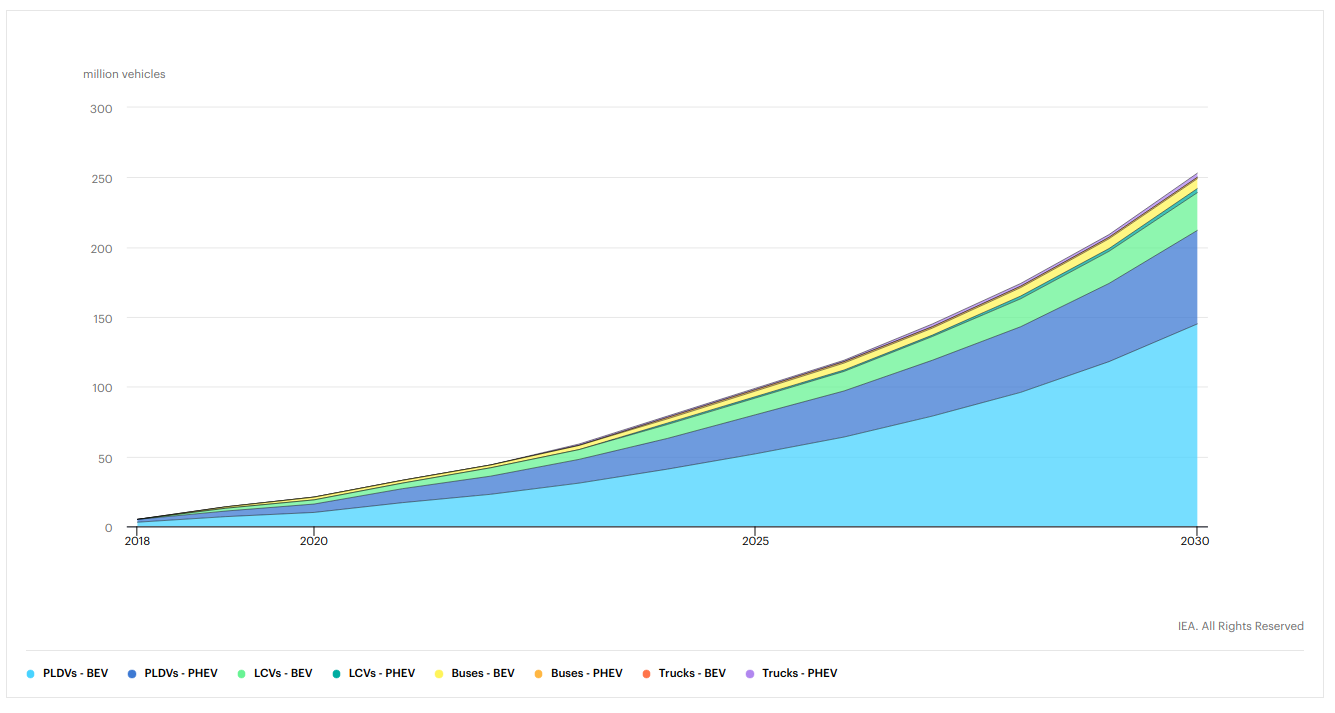
\includegraphics[width=12cm]{ev-scenario-2018-2030.png}\\
    Electric vehicle stock outlook. Source: IEA.org
  \end{center}
  
\end{frame}

\note{%
  
}

\begin{frame}[label=L0]{Application}
  \begin{center}
    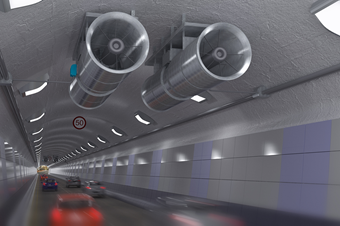
\includegraphics[width=8cm]{fan.png}
  \end{center}

\end{frame}

\note{%
}

\pgfmathsetmacro{\kmotor}{1.7}
\pgfmathsetmacro{\armatureR}{0.5}
\pgfmathsetmacro{\armatureV}{400}
\pgfmathsetmacro{\currentmax}{120}
\pgfmathsetmacro{\Tmax}{\kmotor*\currentmax}
\pgfmathsetmacro{\dragcoeff}{0.002}
\pgfmathsetmacro{\frictioncoeff}{0.1}
\pgfmathsetmacro{\constload}{1}
\pgfkeys{/pgf/fpu}
\pgfmathsetmacro{\bbb}{-1/(-\dragcoeff)*(\kmotor*\kmotor/\armatureR+\frictioncoeff)}
\pgfmathsetmacro{\ccc}{1/(-\dragcoeff)*((\armatureV/\armatureR)*\kmotor - \constload)}
\pgfmathsetmacro{\weq}{-\bbb/2 + 1/2*sqrt(\bbb*\bbb - 4*\ccc)}
\pgfmathsetmacro{\Teq}{\constload + \frictioncoeff*\weq + \dragcoeff*\weq*\weq}
\pgfmathsetmacro{\wminlin}{\armatureV/\kmotor - \Tmax/\kmotor/\kmotor*\armatureR}

\pgfkeys{/pgf/fpu=false}

\begin{frame}[label=L1]{Load torque vs speed}
  \begin{center}
    \begin{tikzpicture}
      \begin{axis}[
        width=8cm,
        height=6cm,
        axis lines = middle,
        ytick=\empty,
        xtick=\empty,
        ylabel={$T_l$},
        xlabel={$\omega$ [rad/s]},
        %ymax=5,
        xmin=0,
        xmax=350,
        ymax=400,]
        \addplot [orange!90!black, smooth, domain=0:300] {sign(x)*(\constload + \frictioncoeff *x + \dragcoeff *x*x)};
      \end{axis}
    \end{tikzpicture}
  \end{center}
      
\end{frame}

\note{%
}

\begin{frame}[label=L2]{Motor torque vs speed}
  With constant armature voltage, and limit on the current, the DC motor will produce a torque dependent on the speed as in the blue plot below. 
  \begin{center}
    \begin{tikzpicture}
      \small
      \begin{axis}[
        width=8cm,
        height=6cm,
        axis lines = middle,
        ytick={0, \Teq, \Tmax},
        yticklabels={0, $T_e$, $T_{max}$},
        xtick={0, \wminlin,\weq},
        xticklabels={0, $\omega_1$, $\omega_e$},
        ylabel={$T$},
        xlabel={$\omega$ [rad/s]},
        %ymax=5,
        xmin=0,
        xmax=300,
        ymax=400,]
        \addplot [orange!90!black, smooth, domain=0:300] {sign(x)*(\constload + \frictioncoeff *x + \dragcoeff *x*x)};
        \addplot [blue!80!black, domain=0:280, samples=120] {(x<\wminlin)*\Tmax + (x>=\wminlin)*(\kmotor*\armatureV/\armatureR - \kmotor*\kmotor/\armatureR * x)};
      \end{axis}
    \end{tikzpicture}
  \end{center}
      
\end{frame}

\note{%
}

\begin{frame}[label=L3E]{Speed vs time}
  \begin{center}
    \begin{tikzpicture}[scale=0.65]
      \tiny
      \begin{axis}[
        width=8cm,
        height=6cm,
        axis lines = middle,
        ytick={0, \Teq},
        %yticklabels={0, $T_e$, $T_{max}$},
        xtick={0,\weq},
        %xticklabels={0, $\omega_1$, $\omega_e$},
        ylabel={$T$},
        xlabel={$\omega$ [rad/s]},
        %ymax=5,
        xmin=0,
        xmax=300,
        ymax=400,]
        \addplot [orange!90!black, smooth, domain=0:300] {sign(x)*(\constload + \frictioncoeff *x + \dragcoeff *x*x)};
        \addplot [blue!80!black, domain=0:280, samples=120] {(x<\wminlin)*\Tmax + (x>=\wminlin)*(\kmotor*\armatureV/\armatureR - \kmotor*\kmotor/\armatureR * x)};
      \end{axis}
    \end{tikzpicture}
  \end{center}

  Given the above motor torque curve and load torque curve, which of the below graphs best describe the response of the speed? 

  \begin{center}
    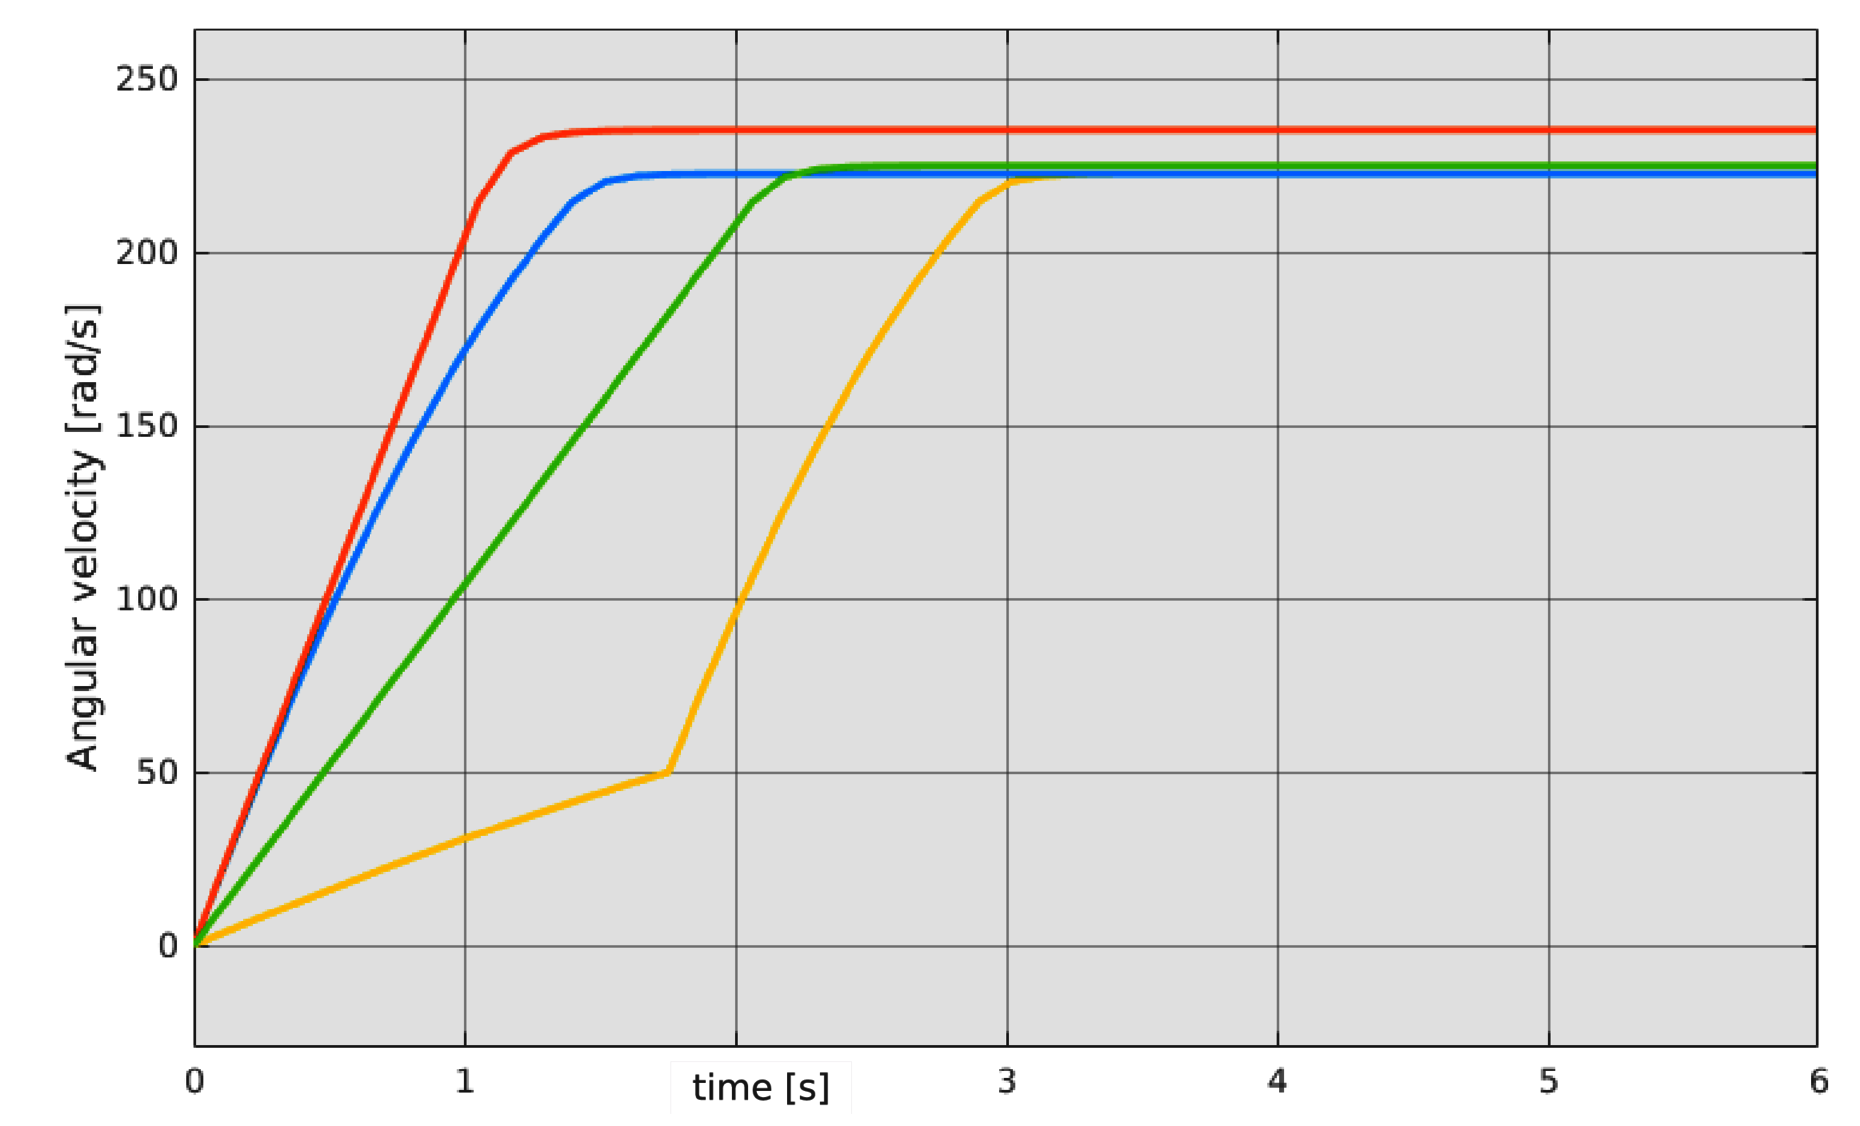
\includegraphics[width=6cm]{./dc-response-crop.png}
  \end{center}
\end{frame}

\note{%
}

\begin{frame}[label=C0]{Cascade-control (two-loop control) of DC motor drives}
\begin{center}
   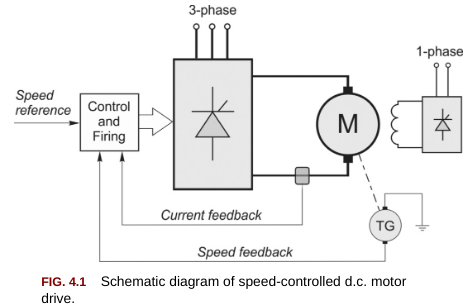
\includegraphics[width=0.6\linewidth]{HD-fig4_1.png}\\
   {\footnotesize Source: Hughes \& Drury}
   \end{center}
\end{frame}

\note{%
}

\begin{frame}[label=C1]{Feedback control}
  \begin{center}
  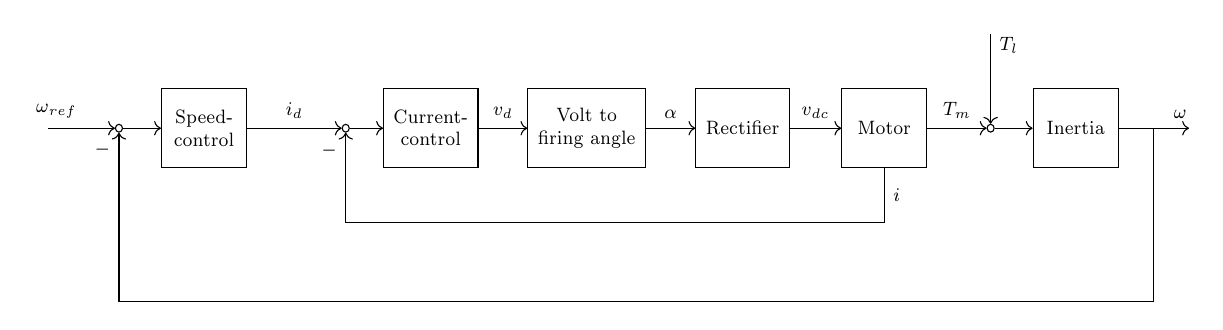
\begin{tikzpicture}[every node/.append style={transform shape}, xscale = 0.9, font=\scriptsize,
block/.style={rectangle, draw, minimum width=12mm, minimum height=10mm, inner sep=4pt},
amp/.style = {regular polygon, regular polygon sides=3,
      draw, fill=white, text width=1em,
      inner sep=1pt, outer sep=0mm,
      shape border rotate=-90},
      summ/.style = {circle, draw, inner sep = 1pt},]
 \node[block,] (motor) at (0,0) {Motor};
 \node[summ, right of=motor, node distance = 15mm,] (sumtorque) {};
 \node[block, right of=sumtorque, node distance=12mm, align=center] (load) {Inertia};
 \node[coordinate, right of=load, node distance = 16mm,] (output) {};
 \node[block, left of=motor, node distance=20mm] (rectifier) {Rectifier};
 \node[block, left of=rectifier, node distance=22mm, align=center] (vtoangle) {Volt to\\firing angle};
 \node[block, left of=vtoangle, node distance=22mm, align=center] (ccontrol) {Current-\\control};
 \node[summ, left of=ccontrol, node distance = 12mm,] (sumcurr) {};
 \node[block, left of=sumcurr, node distance = 20mm, align=center,] (scontrol) {Speed-\\control};
 \node[summ, left of=scontrol, node distance = 12mm,] (sumsp) {};
 \node[coordinate, left of=sumsp, node distance = 10mm,] (setpoint) {};

 \draw[->] (setpoint) -- node[above, very near start ] {$\omega_{ref}$} (sumsp);
 \draw[->] (sumsp) -- node[above, ] {} (scontrol);
 \draw[->] (scontrol) -- node[above, ] {$i_d$} (sumcurr);
 \draw[->] (sumcurr) -- node[above, ] {} (ccontrol);
 \draw[->] (ccontrol) -- node[above, ] {$v_d$} (vtoangle);
 \draw[->] (vtoangle) -- node[above, ] {$\alpha$} (rectifier);
 \draw[->] (rectifier) -- node[above, ] {$v_{dc}$} (motor);
 \draw[->] (motor) -- node[above, ] {$T_m$} (sumtorque);
 \draw[->] (sumtorque) -- node[above, ] {} (load);
 \draw[->] (load) -- node[pos=0.5, coordinate] (meas) {} node[above, very near end] {$\omega$} (output);
 \draw[->] (motor) -- node[right] {$i$} ++(0,-12mm) -| node[pos=0.9, left] {$-$} (sumcurr);
 \draw[->] (meas) -- node[right] {} ++(0,-22mm) -| node[pos=0.95, left] {$-$} (sumsp);
 \draw[<-] (sumtorque) -- node[right, very near end] {$T_l$} ++(0, 12mm);

 %\draw[red, thick] (-80mm, -15mm) rectangle ($ (motor.north east) + (3mm, 10mm) $);
 %\node at ($ (motor.north) + (-10mm, 5mm) $) {$T_m(t) \approx k i_d(t)$};
 \end{tikzpicture}
\end{center}


\end{frame}

\note{%
}

\begin{frame}[label=C2]{Feedback control}
\[ i(t) \approx i_d(t)\]

  \begin{center}
  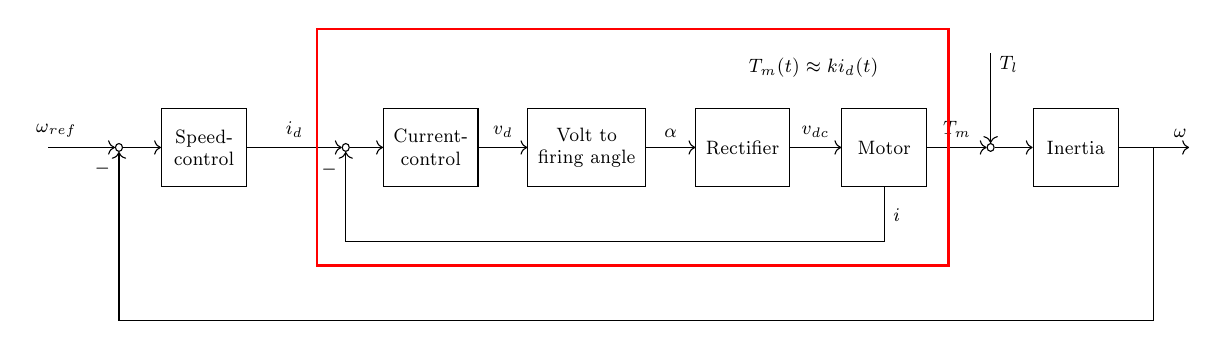
\begin{tikzpicture}[every node/.append style={transform shape}, xscale = 0.9, font=\scriptsize,
block/.style={rectangle, draw, minimum width=12mm, minimum height=10mm, inner sep=4pt},
amp/.style = {regular polygon, regular polygon sides=3,
      draw, fill=white, text width=1em,
      inner sep=1pt, outer sep=0mm,
      shape border rotate=-90},
      summ/.style = {circle, draw, inner sep = 1pt},]
 \node[block,] (motor) at (0,0) {Motor};
 \node[summ, right of=motor, node distance = 15mm,] (sumtorque) {};
 \node[block, right of=sumtorque, node distance=12mm, align=center] (load) {Inertia};
 \node[coordinate, right of=load, node distance = 16mm,] (output) {};
 \node[block, left of=motor, node distance=20mm] (rectifier) {Rectifier};
 \node[block, left of=rectifier, node distance=22mm, align=center] (vtoangle) {Volt to\\firing angle};
 \node[block, left of=vtoangle, node distance=22mm, align=center] (ccontrol) {Current-\\control};
 \node[summ, left of=ccontrol, node distance = 12mm,] (sumcurr) {};
 \node[block, left of=sumcurr, node distance = 20mm, align=center,] (scontrol) {Speed-\\control};
 \node[summ, left of=scontrol, node distance = 12mm,] (sumsp) {};
 \node[coordinate, left of=sumsp, node distance = 10mm,] (setpoint) {};

 \draw[->] (setpoint) -- node[above, very near start ] {$\omega_{ref}$} (sumsp);
 \draw[->] (sumsp) -- node[above, ] {} (scontrol);
 \draw[->] (scontrol) -- node[above, ] {$i_d$} (sumcurr);
 \draw[->] (sumcurr) -- node[above, ] {} (ccontrol);
 \draw[->] (ccontrol) -- node[above, ] {$v_d$} (vtoangle);
 \draw[->] (vtoangle) -- node[above, ] {$\alpha$} (rectifier);
 \draw[->] (rectifier) -- node[above, ] {$v_{dc}$} (motor);
 \draw[->] (motor) -- node[above, ] {$T_m$} (sumtorque);
 \draw[->] (sumtorque) -- node[above, ] {} (load);
 \draw[->] (load) -- node[pos=0.5, coordinate] (meas) {} node[above, very near end] {$\omega$} (output);
 \draw[->] (motor) -- node[right] {$i$} ++(0,-12mm) -| node[pos=0.9, left] {$-$} (sumcurr);
 \draw[->] (meas) -- node[right] {} ++(0,-22mm) -| node[pos=0.95, left] {$-$} (sumsp);
 \draw[<-] (sumtorque) -- node[right, very near end] {$T_l$} ++(0, 12mm);

 \draw[red, thick] (-80mm, -15mm) rectangle ($ (motor.north east) + (3mm, 10mm) $);
 \node at ($ (motor.north) + (-10mm, 5mm) $) {$T_m(t) \approx k i_d(t)$};
 \end{tikzpicture}
\end{center}

\end{frame}

\note{%
}

\begin{frame}[label=C3]{PI-control}
\[ i(t) \approx i_d(t)\]

  \begin{center}
  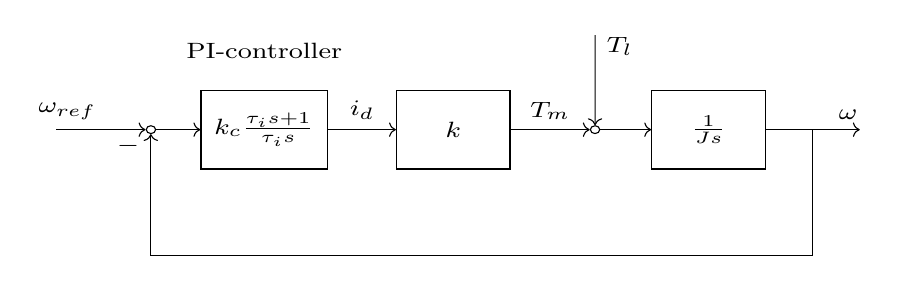
\begin{tikzpicture}[every node/.append style={transform shape}, xscale = 1.2, font=\footnotesize,
block/.style={rectangle, draw, minimum width=12mm, minimum height=10mm, inner sep=4pt},
amp/.style = {regular polygon, regular polygon sides=3,
      draw, fill=white, text width=1em,
      inner sep=1pt, outer sep=0mm,
      shape border rotate=-90},
      summ/.style = {circle, draw, inner sep = 1pt},]
 \node[block,] (motor) at (0,0) {$k$};
 \node[summ, right of=motor, node distance = 15mm,] (sumtorque) {};
 \node[block, right of=sumtorque, node distance=12mm, align=center] (load) {$\frac{1}{Js}$};
 \node[coordinate, right of=load, node distance = 16mm,] (output) {};
 \node[block, left of=motor, node distance=20mm] (pi) {$k_{c}\frac{\tau_{i}s + 1}{\tau_{i}s}$};
 \node[summ, left of=pi, node distance = 12mm,] (sumsp) {};
 \node[coordinate, left of=sumsp, node distance = 10mm,] (setpoint) {};

 \draw[->] (setpoint) -- node[above, very near start ] {$\omega_{ref}$} (sumsp);
 \draw[->] (sumsp) -- node[above, ] {} (pi);
 \draw[->] (pi) -- node[above, ] {$i_d$} (motor);
 \draw[->] (motor) -- node[above, ] {$T_m$} (sumtorque);
 \draw[->] (sumtorque) -- node[above, ] {} (load);
 \draw[->] (load) -- node[pos=0.5, coordinate] (meas) {} node[above, very near end] {$\omega$} (output);
 \draw[->] (meas) -- node[right] {} ++(0,-16mm) -| node[pos=0.95, left] {$-$} (sumsp);
 \draw[<-] (sumtorque) -- node[right, very near end] {$T_l$} ++(0, 12mm);

 \node[above of=pi, node distance=10mm] {PI-controller};
 \end{tikzpicture}
\end{center}

\[\Omega(s)  = \frac{kk_c(\tau_is + 1)}{\tau_iJs^2 + kk_c(\tau_is + 1)}\Omega_{ref}(s) + 
\frac{\tau_is}{\tau_iJs^2 + kk_c(\tau_is + 1)}T_l(s)\] 

\alert{Question:} What it the static gain ($s=0$) for the two input signals \(\omega_{ref}\) and \(T_l\)?

\end{frame}


\note{%
}

\begin{frame}[label=C4E]{System poles and time-response}
For a second-order closed-loop transfer function 
\[  G_c(s) = \frac{K}{s^2 + \frac{1}{2}s + K}\]
and four different choices of $K$, four different pairs of closed-loop poles are obtained.  Pair the poles with the corresponding time-response.
\begin{center}
  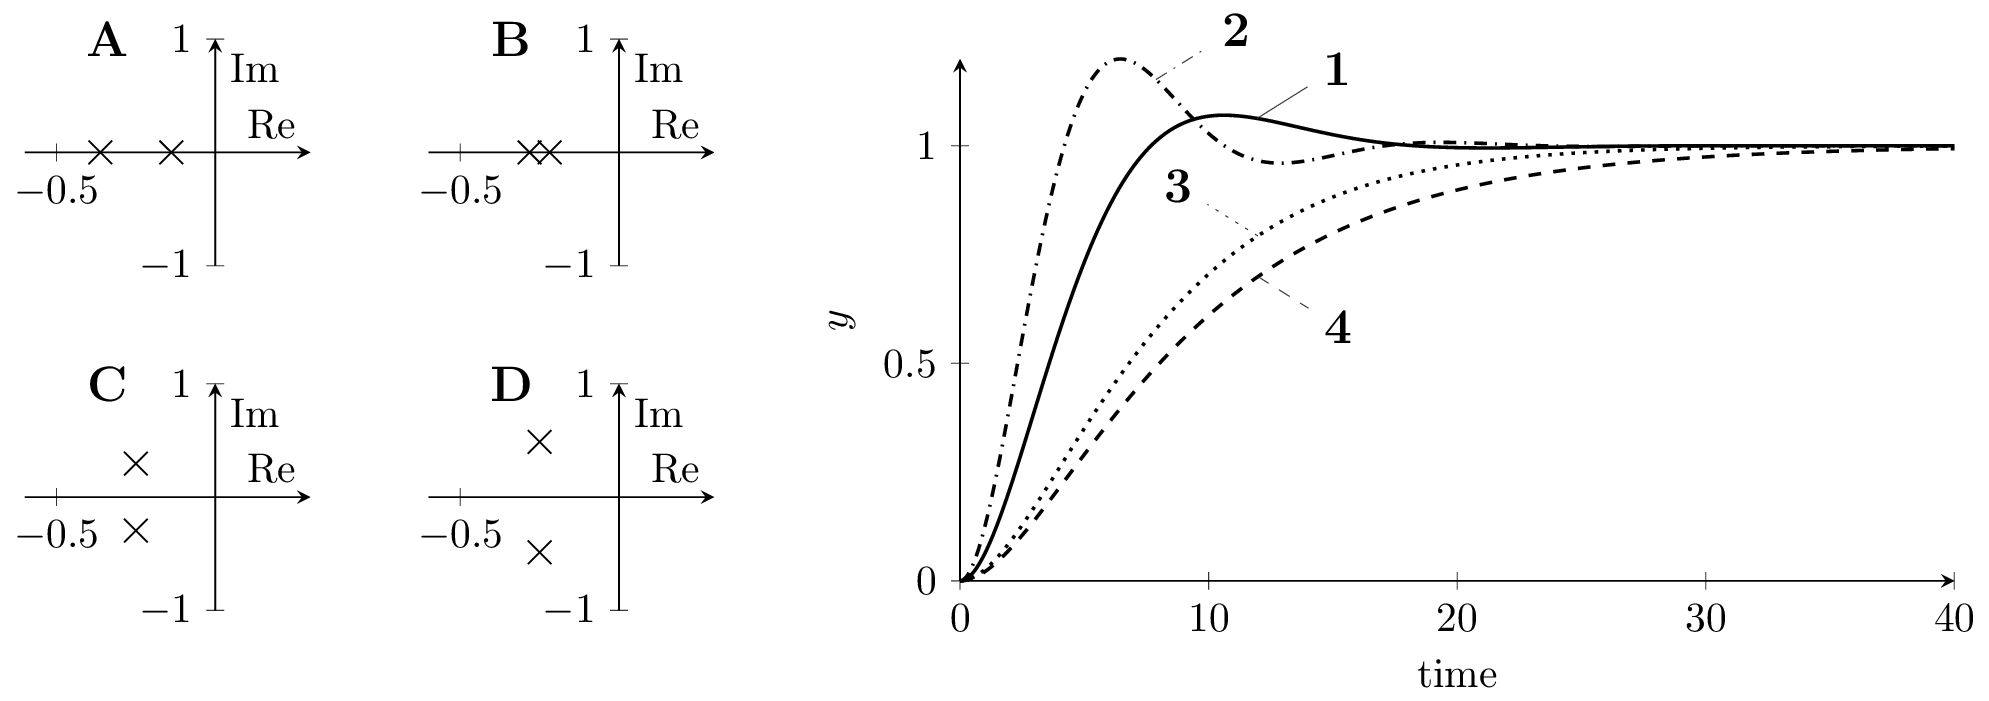
\includegraphics[width=0.77\linewidth]{cstr-control-step-beamer.png}
\end{center}
\end{frame}

\note{%
}

\begin{frame}[label=C5]{Root locus}
  \begin{center}
    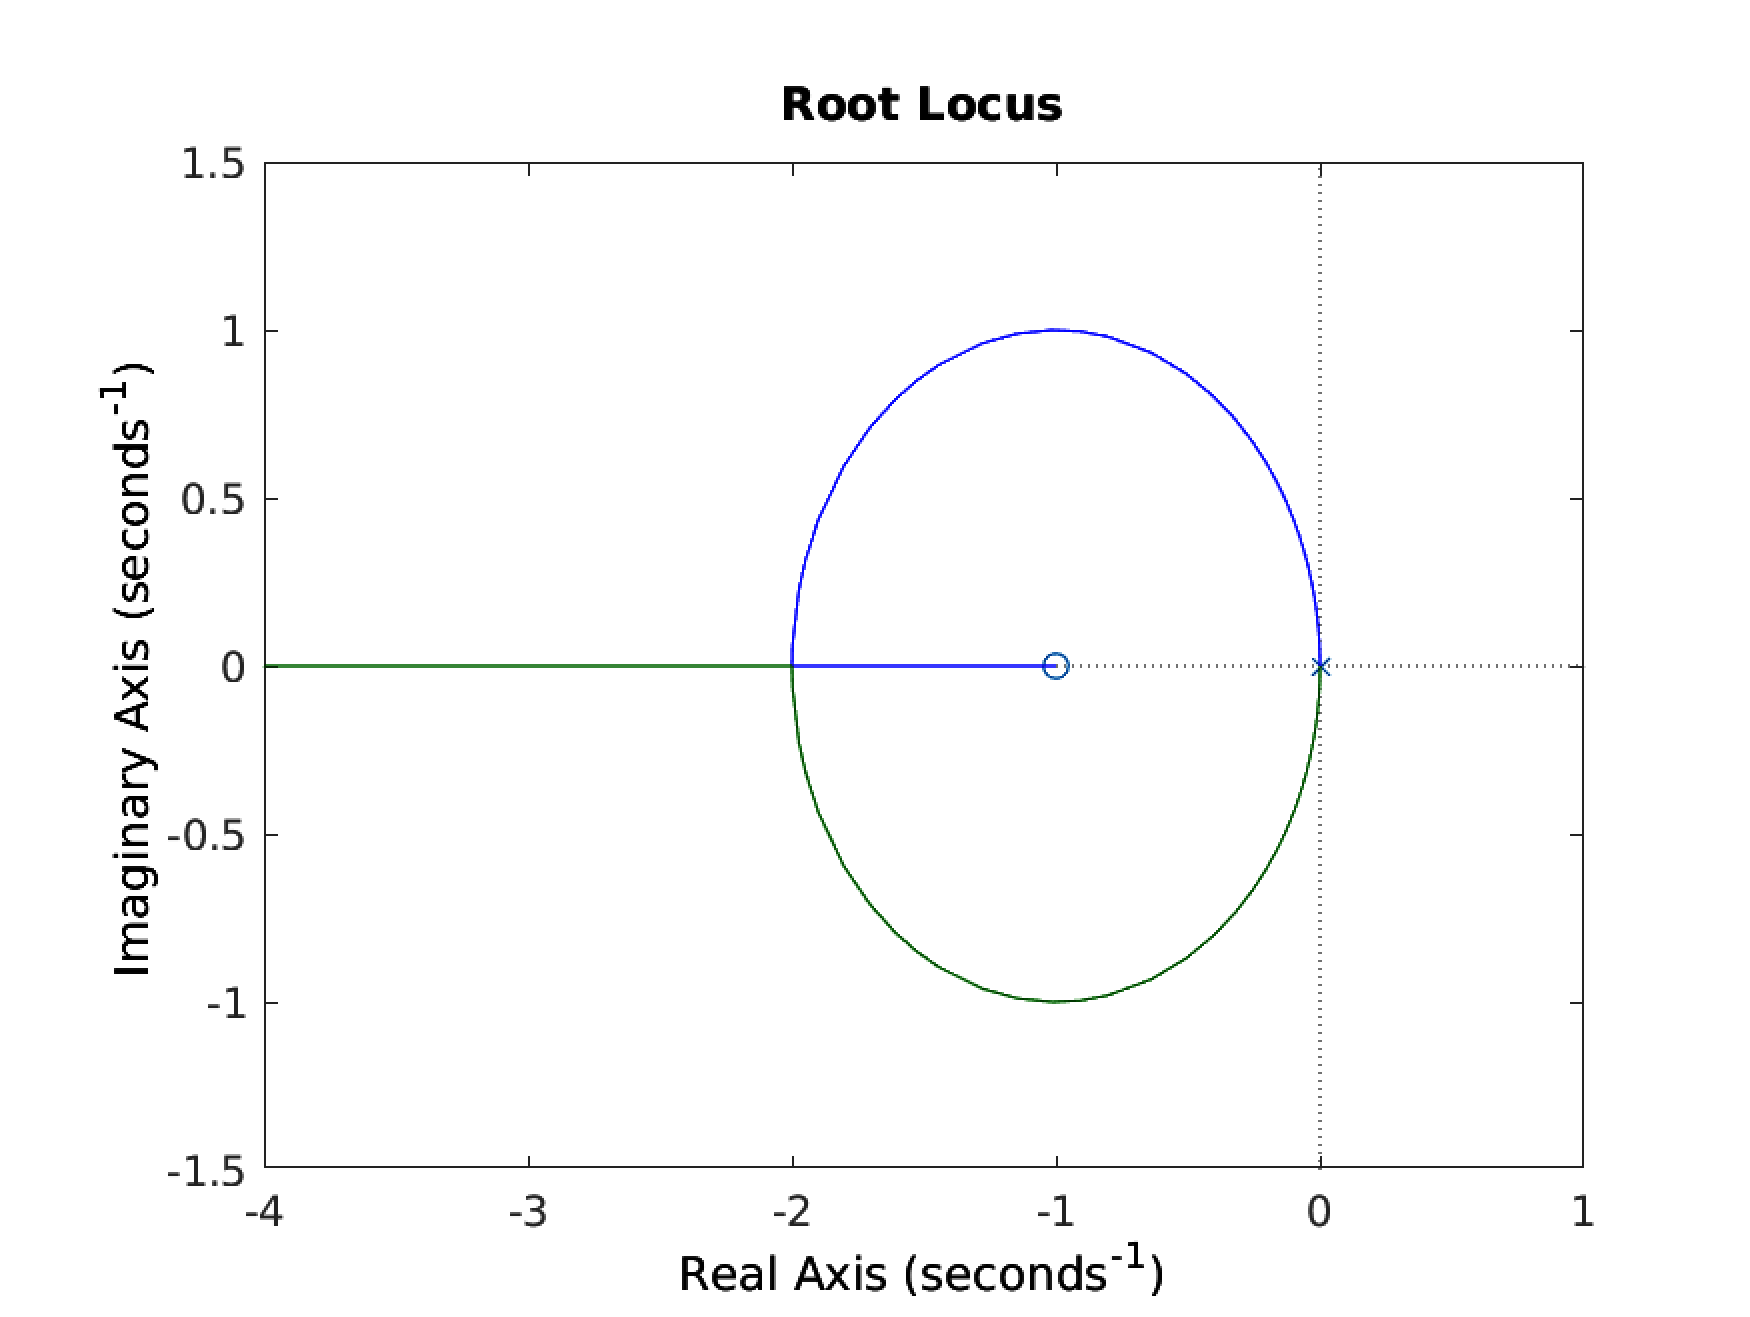
\includegraphics[width=8cm]{rlocus-PI-integrator.png}\\
  \end{center}
  Characteristic equation
  \[ s^2 + k_c\frac{k}{J\tau_i}(\tau_is + 1)= 0. \qquad \text{Root locus for the case}\; \tau_i = 1\]

\end{frame}

\begin{frame}[label=C5E]{Polynomial design}
  Given closed-loop characteristic polynomial
  \[ A_{c} =  s^2 + \frac{k_c k}{J}s + \frac{k_c k}{\tau_i J}\]

  and desired characteristic polynomial (desired poles $p_1$ and $p_2$)

  \[ A_{cd}=(s-p_1)(s-p_2) = s^2 - (p_1+p_2)s + p_1p_2 \]

  We want \(A_c \equiv A_{cd}\).
  
  \alert{Determine} a system of two equations in the two unknown controller parameters $\tau_i$ and $k_c$ by setting the corresponding coefficients equal in both polynomials. \alert{Solve} for $\tau_i$ and $k_c$ in the particular case that \(p_1=p_2=-\frac{1}{\tau_c}\). 
  
\end{frame}

\note{%
}

\begin{frame}[label=W1]{Anti-windup}
     \begin{center}
	  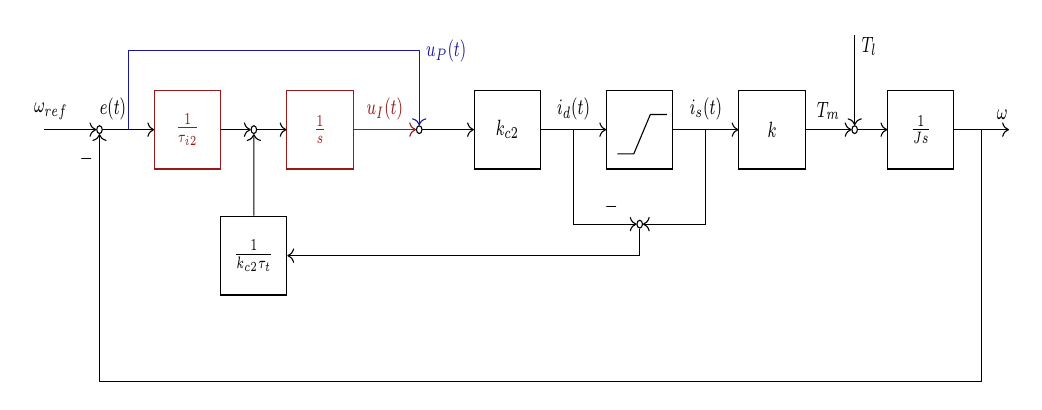
\begin{tikzpicture}[every node/.append style={transform shape}, xscale = 0.7, font=\footnotesize,
	block/.style={rectangle, draw, minimum width=12mm, minimum height=10mm, inner sep=4pt},
	amp/.style = {regular polygon, regular polygon sides=3,
              draw, fill=white, text width=1em,
              inner sep=1pt, outer sep=0mm,
              shape border rotate=-90},
	      summ/.style = {circle, draw, inner sep = 1pt},]
	 \node[block,] (motor) at (0,0) {$k$};
	 \node[summ, right of=motor, node distance = 15mm,] (sumtorque) {};
	 \node[block, right of=sumtorque, node distance=12mm, align=center] (load) {$\frac{1}{Js}$};
	 \node[coordinate, right of=load, node distance = 16mm,] (output) {};
	 \node[block, left of=motor, node distance=24mm] (saturation) {};

	 \node[block, left of=saturation, node distance=24mm] (gain)  {$k_{c2}$};
	 
	 \node[summ, left of=gain, node distance=16mm] (sum2) {};
	 \node[color=iic,block, left of=sum2, node distance=18mm] (int)  {$\frac{1}{s}$};
	 \node[summ, left of=int, node distance=12mm] (sumint) {};
	 \node[color=iic,block, left of=sumint, node distance=12mm] (ii)  {$\frac{1}{\tau_{i2}}$};
	 \node[color=ppc, coordinate, above of=ii, node distance=10mm] (pp)  {};
	 \node[summ, left of=ii, node distance=16mm] (sumsp) {};
	 \node[coordinate, left of=sumsp, node distance = 10mm,] (setpoint) {};

       \draw[->] (sumsp) -- node[above, pos=0.2] {$e(t)$} node[coordinate] (mm) {}  (ii);
       \draw[->] (gain) -- node[coordinate] (idmeas) {} node[above, ] {$i_d(t)$} (saturation);
       \draw[->, color=ppc] (mm) |- (pp) -| node[right,] {$u_P(t)$} (sum2);
       \draw[->, color=iic] (int)  -- node[above,] {$u_I(t)$} (sum2);
       \draw[->] (sum2) -- node[above, near end] {} (gain);



	 \draw[->] (setpoint) -- node[above, very near start ] {$\omega_{ref}$} (sumsp);
	 \draw[->] (saturation) -- node[coordinate, ] (satmeas) {} node[above,] {$i_s(t)$} (motor);
	 \draw[->] (motor) -- node[above, ] {$T_m$} (sumtorque);
	 \draw[->] (sumtorque) -- node[above, ] {} (load);
	 \draw[->] (load) -- node[pos=0.5, coordinate] (meas) {} node[above, very near end] {$\omega$} (output);
	 \draw[->] (meas) -- node[right] {} ++(0,-32mm) -| node[pos=0.95, left] {$-$} (sumsp);
	 \draw[<-] (sumtorque) -- node[right, very near end] {$T_l$} ++(0, 12mm);

	 % Anti-windup
	 \draw ($ (saturation.south west) + (2mm, 2mm) $) -- ++(3mm, 0) -- ++(3mm, 5mm) -- ++(3mm, 0);
	 \node[block, below of=sumint, node distance=16mm] (back) {$\frac{1}{k_{c2}\tau_t}$};
	 \node[summ, below of=saturation, node distance=12mm] (sumsat) {};
	 \draw[->] (satmeas) |- node[above, pos=0.8] {} (sumsat);
	 \draw[->] (idmeas) |- node[above, pos=0.8] {$-$} (sumsat);
	 \draw[->] (sumsat) |- (back);
	 \draw[->] (back) -- (sumint);
	 \draw[->] (ii) -- (sumint);
	 \draw[->] (sumint) -- (int);
	 

	 \node[coordinate, right of=back, node distance=2cm] (sat) {};
  
\end{tikzpicture}
\end{center}


\end{frame}

\note{%
}

\begin{frame}[label=W2E]{Anti-windup exercise}
\end{frame}

\note{%
}

\begin{frame}[label=R1]{Controlling the armature voltage}
\end{frame}

\note{%
}

\pgfmathsetmacro{\cheight}{8}
\pgfmathsetmacro{\cwidth}{5}
\pgfmathsetmacro{\chmid}{0.5*\cheight}
\pgfmathsetmacro{\chtth}{0.67*\cheight}
\pgfmathsetmacro{\chth}{0.25*\cheight}
\pgfmathsetmacro{\swx}{0.5*\cwidth}
\pgfmathsetmacro{\swxx}{0.7*\cwidth}
\pgfmathsetmacro{\swy}{0.5*\chmid}
\pgfmathsetmacro{\diody}{0.8*\cheight}
\pgfmathsetmacro{\diodyy}{0.2*\cheight}
\pgfmathsetmacro{\capx}{0.6*\cwidth}
\begin{frame}[label=R2]{Controlled rectifier circuit}
\begin{columns}
\begin{column}{0.3\columnwidth}
	\begin{center}
	  \begin{circuitikz}[american, scale=0.7, transform shape]
            \draw (\cwidth, \chth) node[elmech](motor){M};
	    \draw (0, \cheight) to[sV=$V$] (0,0);
	    \draw (0, \cheight) to[thyristor, l_=T1] (\swx, \cheight) to[short] (\cwidth, \cheight)
	    to[R=$R$, i=$i$,] (\cwidth, \chtth) to[L=$L$] (motor.north);
            \draw (motor.south) to (\cwidth, 0);
	    \draw (\cwidth,0) to[short] (\swx, 0) to[thyristor, l_=T4] (0, 0);
	    \draw[] (0, 1) to[short] (1, 1) to[short] (1, \diody) to[thyristor, l_=T2] (\swxx, \diody)
	    to[short] (\swxx, \cheight);
	    \draw[] (\swxx, 0) to[short] (\swxx, \diodyy) to[thyristor, l_=T3] (1.5, \diodyy) to[short] (1.5, 4) to[crossing] (0.5, 4) to[short] (0, 4);
	  \end{circuitikz}
	\end{center}
\end{column}

\begin{column}{0.7\columnwidth}

\begin{center}
  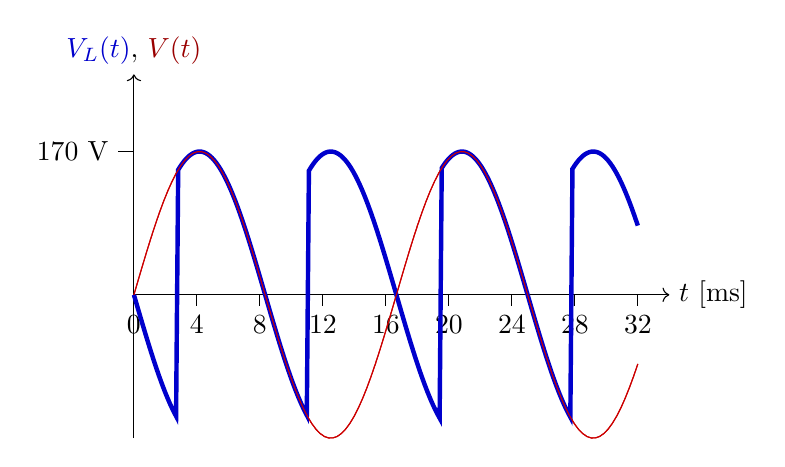
\begin{tikzpicture}[xscale=0.2]
  \pgfmathsetmacro{\alppha}{60}
  \begin{scope}[yscale=1.4]

  \draw[->] (0, 0) -- (34, 0) node[right] {$t$ [ms]};
    \draw[->] (0, -1.3) -- (0, 2) node[above] {$\textcolor{blue!80!black}{V_L(t)}, \, \textcolor{red!60!black}{V(t)}$};
    \draw (0, 1.3) -- (-1, 1.3) node[left] {170 V};
    \foreach \t in {0, 4, 8, ..., 32} {
    \draw (\t, 0) -- (\t, -0.1) node[below] {\t};
    }
    \draw[red!80!black,domain = 0:32, samples=120] plot (\x, {1.3*sin((60/1000*360)*\x)});
    \draw[ultra thick,blue!80!black,domain = 0:32, samples=240] plot (\x, {-(Mod((60/1000*360)*\x, 360) < \alppha))*1.3*sin((60/1000*360)*\x) + (Mod((60/1000*360)*\x, 360) > \alppha)*(Mod((60/1000*360)*\x, 360) < 180+\alppha)*1.3*sin((60/1000*360)*\x) - (Mod((60/1000*360)*\x, 360) > 180+\alppha)*(Mod((60/1000*360)*\x, 360) < 360)*1.3*sin((60/1000*360)*\x)});
    \draw[thin, red!80!black,domain = 0:32, samples=120] plot (\x, {1.3*sin((60/1000*360)*\x)});
    \end{scope}
    \end{tikzpicture}

\end{center}
\end{column}
\end{columns}

\end{frame}

\note{%
}

\begin{frame}[label=R3A]{Rectified voltage dependency on firing angle}
  \begin{center}
  \begin{animateinline}[controls, palindrome]{2}
      \multiframe{13}{n=0+15}{
        \begin{circuitikz}[scale=0.7, american]
          %\useasboundingbox (-1 cm, -1 cm) rectangle (9 cm, 3 cm);
	  \begin{scope}[yshift=5cm, scale=0.5, transform shape]
            \draw (\cwidth, \chth) node[elmech](motor){M};
	    \draw (0, \cheight) to[sV=$V$] (0,0);
	    \draw (0, \cheight) to[thyristor, l_=T1] (\swx, \cheight) to[short] (\cwidth, \cheight)
	    to[R=$R$, i=$i$] (\cwidth, \chtth) to[L=$L$] (motor.north);
            \draw (motor.south) to (\cwidth, 0);
	    \draw (\cwidth,0) to[short] (\swx, 0) to[thyristor, l_=T4] (0, 0);
	    \draw[] (0, 1) to[short] (1, 1) to[short] (1, \diody) to[thyristor, l_=T2] (\swxx, \diody)
	    to[short] (\swxx, \cheight);
	    \draw[] (\swxx, 0) to[short] (\swxx, \diodyy) to[thyristor, l_=T3] (1.5, \diodyy) to[short] (1.5, 4) to[crossing] (0.5, 4) to[short] (0, 4);
	  \end{scope}

          \begin{axis}[%
            width=4cm,
            height=4cm,
            xtick=\empty,
            ytick={0, 30, 60, 90, 120, 150, 180},
            ylabel={Firing angle},
            ]
            \addplot[green!80!black, domain=0:12] {15*x};
            \addplot[red!80!black] coordinates {(0, \n) (12, \n)};
          \end{axis}

          \begin{axis}[%
            yshift=4.5cm,
            xshift=4.5cm,
            width=9cm,
            height=5cm,
            xtick=\empty,
            axis lines=middle,
            %ytick={0, 30, 60, 90, 120, 150},
            ylabel={Voltage},
            ymin=-600,
            ymax=1200,
            clip=false,
            ]
            \addplot[blue!80!black, solid, thick, smooth] table[col sep = comma, y index =1] {alpha_volt_current_\n.dta};
            \addplot[magenta!70, solid] table[col sep = comma, y index =2] {alpha_volt_current_\n.dta};
          \end{axis}

          \begin{axis}[%
            yshift=0cm,
            xshift=4.5cm,
            width=9cm,
            height=5cm,
            xtick=\empty,
            axis lines=middle,
            %ytick={0, 30, 60, 90, 120, 150},
            ylabel={Current},
            xlabel={Time},
            ymin=-10,
            ymax=250,
            ]
            \addplot[orange!80!black, solid, thick, smooth] table[col sep = comma, y index =3] {alpha_volt_current_\n.dta};
            \addplot[yellow!80!black, solid] table[col sep = comma, y index =4] {alpha_volt_current_\n.dta};
          \end{axis}

          
        \end{circuitikz}
        %\end{tikzpicture}
      }
    \end{animateinline}
  \end{center}


\end{frame}

\note{%
}


\begin{frame}[label=R3E]{Rectified voltage dependency on firing angle}

  \begin{center}
    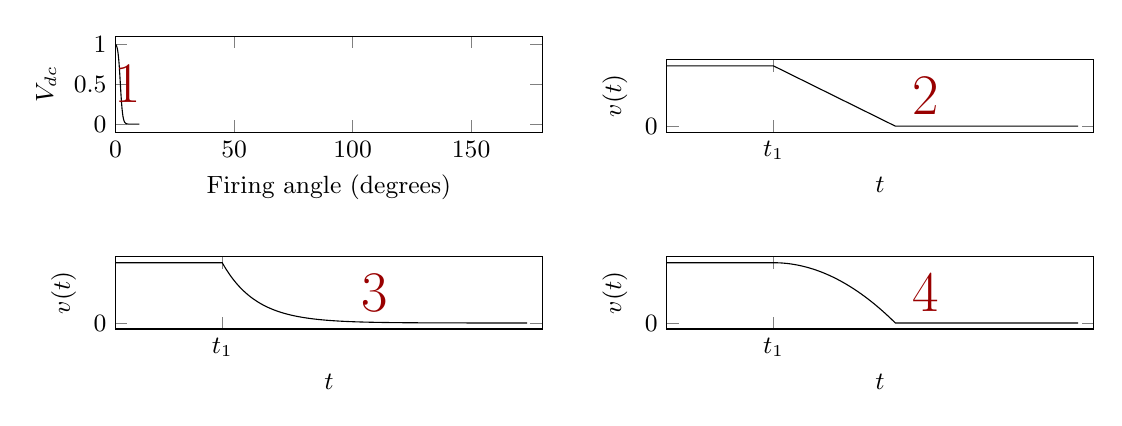
\begin{tikzpicture}
      \small

      \begin{axis}[
        width=7cm,
        height=2.8cm,
        xlabel={Firing angle (degrees)},
        ylabel={$V_{dc}$},
        xmin=0,
        xmax=180,
        %ytick = {0},
        %xtick = {0},
        ]
        \addplot+[black, no marks, domain=-4:10, samples=400,variable=k] { (k < 0) + (k>0)*(1+exp(-4))/(1+exp(4*(0.5*k-1)))};

        \node[black!40!red] at (axis cs: 5, 0.5) {\huge 1};
      \end{axis}

      \begin{axis}[
        xshift=7cm,
        width=7cm,
        height=2.5cm,
        xlabel={$t$},
        ylabel={$v(t)$},
        xmin=-3.5,
        xmax=10.5,
        ytick = {0},
        xtick = {0},
        xticklabels = {$t_1$},
        ]
        \addplot+[black, no marks, domain=-4:10, samples=400,variable=k] { (k<0) + ((k>=0) - (k>4))*(1/4*(4-k)) };
        \node[black!40!red] at (axis cs: 5, 0.5) {\huge 2};
      \end{axis}

      \begin{axis}[
        xshift=0cm,
        yshift=-2.5cm,
        width=7cm,
        height=2.5cm,
        xlabel={$t$},
        ylabel={$v(t)$},
        xmin=-3.5,
        xmax=10.5,
        ytick = {0},
        xtick = {0},
        xticklabels = {$t_1$},
        ]
        \addplot+[black, no marks, domain=-4:10, samples=400,variable=k] { (k<0) + (k>0)*exp(-0.9*k)};
        \node[black!40!red] at (axis cs: 5, 0.5) {\huge 3};
      \end{axis}

      \begin{axis}[
        xshift=7cm,
        yshift=-2.5cm,
        width=7cm,
        height=2.5cm,
        xlabel={$t$},
        ylabel={$v(t)$},
        xmin=-3.5,
        xmax=10.5,
        ytick = {0},
        xtick = {0},
        xticklabels = {$t_1$},
        ]
        \addplot+[black, no marks, domain=-4:10, samples=400,variable=k] { (k<0) + ((k>=0) - (k>4))*(1-1/16*pow(-k,2)) };
        \node[black!40!red] at (axis cs: 5, 0.5) {\huge 4};
      \end{axis}


    \end{tikzpicture}

  \end{center}



\end{frame}

\note{%
}

\end{document}
